\documentclass[a4paper,11pt]{article}

\usepackage[italian]{babel}

\usepackage[latin1]{inputenc}

\usepackage[T1]{fontenc}

\usepackage{graphicx}

\usepackage{indentfirst}

\usepackage{amsmath,amssymb}

\usepackage{enumitem} 

\newcommand{\virgolette}[1]{``#1''}

\usepackage[margin=1in]{geometry} %Smaller margins

\usepackage{lmodern} %Vector PDF

\usepackage{siunitx}

\usepackage{xcolor}

\usepackage{colortbl}

\usepackage{multirow}

\usepackage{rotating}

\usepackage{booktabs}

\usepackage{longtable}

\usepackage{graphicx}
\graphicspath{ {Images/} }

\usepackage{wrapfig}

\newcommand*\chem[1]{\ensuremath{\mathrm{#1}}}

\begin{document}

L'interferometro di Michelson è uno strumento che sfrutta alcune proprietà delle radiazioni luminose per metternee in evidenza alcune caratteristiche. In particolare sfruttando una combinazione di specchi semiriflettenti e altri completamente riflettenti, come mostrato in figura \ref{interf} è possibile individuare la lunghezza d'onda di una particolare sorgente a partire dalla figura di interferenza che risulta.

\begin{figure}[htpb]
	\centering
	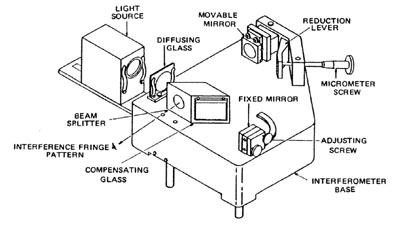
\includegraphics[scale=0.8]{/../../Immagini/interf}
	\caption{Schema della composizione e del funzionamento di un interferometro di Michelson.}\label{interf}
\end{figure}	

La relazione che lega infatti la lunghezza d'onda $\lambda$ della sorgente, alla figura che si osserva muovendo uno dei due specchi riflettenti è la seguente:
\begin{equation}\label{lambda}
\lambda=\dfrac{2n_a\Delta x}{N_1}
\end{equation}
dove $n_a$ rappresenta l'indice di rifrazione dell'aria, $\Delta x$ indica lo spostamento di una delle due lenti e $N_1$ è il numero di massimi (o equivalentemente minimi) osservati mentre si spostava lo specchio di $\Delta x$.

Quello che si osserva è che questa relazione consente di calcolare il valore di $\lambda$ a patto di conoscere il valore dell'indice di rifrazione $n_a$. Questo pu\'o a sua volta essere ricavato utilizzando una camera di lunghezza $d$ in cui viene creato il vuoto, contando le frange che si susseguono quando questa viene riportata alle condizioni dell'ambiente circostante. Vale infatti la relazione:
\begin{equation}\label{indice_aria}
	2 (n_a - 1) d = N_2 \lambda
\end{equation}
dove $1$ è l'indice di rifrazione del vuoto, e $N_2$ è il numero di frange che si sono susseguite.

Mettendo a sistema \ref{lambda} e \ref{indice_aria} si ricavano i valori sia di $\lambda$ che di $n_a$.

Queste relazioni sono tanto pi\'u evidenti quanto lo spettro che emette verso l'interferometro si avvicina alla condizione di monocromaticità. Per luce non monocromatica, come una sorgente \virgolette{bianca} tramite un interferometro è possibile ricavare la lunghezza del pacchetto d'onda -- dato dalla sovrapposizione delle varie lunghezze d'onda emesse. Infatti è possibile con un po di attenzione osservare in maniera diretta la lunghezza di un pacchetto di luce emessa.

Allo stesso modo è possibile risolvere due lunghezze d'onda apparentemente molto vicine tra loro come nel caso del doppietto di sodio, sfruttando la relazione:
\begin{equation}\label{delta1}
	\Delta_1=2N_1\frac{\lambda_1}{2}=(2N_1+1)\frac{\lambda_2}{2}
\end{equation}
dove $\Delta_1$ è la differenza di cammino ottico tra le due lunghezze d'onda ed $N_1$ l'intero che meglio soddisfa la relazione 
\[
N_1 = \dfrac{\lambda_1}{2(\lambda_2 - \lambda_1)}\]
\end{document}